\section{Introduction}
\label{sec:intro}

{ \color{red}
    Emphasize the hypothesis generation, remove references to OLAP}

Consider a data warehouse scenario: a database describes how a set of
\emph{measures} varies along several \emph{dimensions}. To work with this
database, analysts need a lot of prior knowledge: which dimensions and measures
they are interested in, where interesting patterns are hidden in the cube,
which dependencies among dimensions and measures exist, and much more.  Manual
exploration may expose some of this knowledge, but its success depends entirely
on chance and intuition. In contrast, we aim at a semi-automated exploration.
We want to assist the humans in understanding how measures are distributed,
where unexpected measures appear, and where interesting dependencies between
dimensions and measures arise.

We believe that automating query generation is essential to make analysts more
productive. Informations which are trivial for domain experts are not
necessarily so for data specialists. Besides, experts themselves may need
guidance. Consider for instance Figure \ref{intro}. The table shows a small
extract from a dataset of astronomical observations\footnote{This dataset come
from the LOFAR research programme, 21 May 2012, the Netherlands}. We want to
observe the \emph{brightness} of more than 100,000 sources, taken at different
times, frequency ranges and with different precisions. In total, there are more
than fifty dimensions. Even for an astronomer, this dataset cannot be
understood by intuition alone. We need intelligent tools to provide guidance.
The bottom picture illustrates what we expect from our query generation system:
a simpler low dimension view of dependent dimensions and measures.  Anyone can
quickly perceive bright regions.

Semi-automated exploration of data cubes is fundamentally challenging for two
reasons. The first reason is obvious: how do we recognize ``interesting''
queries?  The diversity of opinions in the literature is rather depressing.
What is interesting for a user can be extremely boring for another. The second
problem is practical.  Suppose that we had a universal measure of interest, how
could we explore the search space fast enough to find the interesting queries?

Many authors have proposed semi-automated (or discovery-driven) exploration
frameworks in the past. Typically, they introduce a fixed ``interestingness''
model, then the exploit the particularities of their model to speed up
computations.  For instance, a seminal work was presented by Sarawagi et al.
\cite{sarawagi1998discovery}. According to their paper, the most interesting
queries are the most ``surprising'' ones.  They suggest to build a (log-linear)
model over the data, and identify the largest deviations. More recently, Dash
et al.\cite{dash2008dynamic} proposed a facet selection method, also based on
surprise. Nevertheless, given the diversity of users and requirements, are
these interestingness models \emph{really} interesting?

In this paper, we introduce \textit{Claude}, a generic query generation
system. \emph{Claude lets users describe what they are looking for.
Given their input, it explores the database and reveals interesting OLAP views}.
Here is how it operates. First, the users assign a value to each tuple in
the database.  We call this value the \emph{target}. It can come from the raw
data (e.g., the brightness of light sources), a calculation (e.g., a
``surprise'' score from the litterature), or manual effort. Claude's job is to
present the ``big picture'': it explains how the target is distributed across
the database, and what influences it. To do so, it operates in two steps.
First, it explores the database for interesting projections. Then, for each
projection, it reveals ``remarkable'' areas. 

Making Claude efficient is a major challenge. We
introduce two algorithms.  The first one is exact and based on a systematic
level-wise search paradigm.  The second one is a much faster and based on a
relaxation of our model and a heuristic search.

\section{Presentation and Objectives}

\subsection{Overview}
\begin{figure}[t!]
\centering
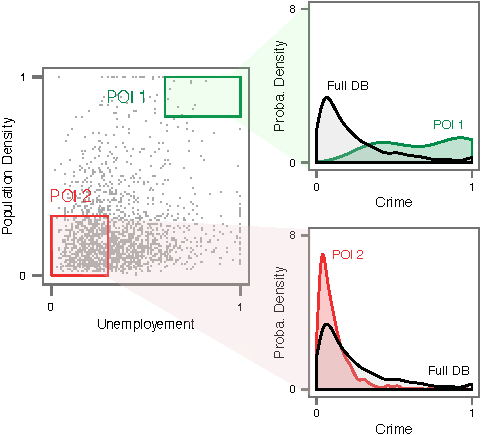
\includegraphics[width=\columnwidth]{images/Overview}
\caption{Example of explanation, with two points of interest. All the values
are normalized.}
\label{fig:overview}
\end{figure}
We represent the database by a large table $DB$. This table contains two types
of columns: the dimensions $X_0, \ldots, X_N$ and a target column $T$. This
view is logical, we are oblivious to the physical structure of the data.
Claude's aim is to describe what causes the target to vary. To do so, it
generates \textbf{explanations}.  An explanation is a set of two elements: a
\textbf{view} and a list of \textbf{points of interest} (POI). A view is an
``interesting'' set of columns.  More exactly, it is a set of columns which
have a strong \emph{influence} on the target. A POI is a region where this
influence is maximal, and thus the target takes unusual values.

We illustrate these notions with a running example. We want to understand what
causes crime in US communities. We have a database of cities with several dozen
socio-economic indicators (for instance, employment, age, or diplomas). For
each city we also have the annual number of violent crimes: this is our target
variable. This example comes from a real use case, which we will
present in Section \ref{sec:crime}.

Figure~\ref{fig:overview} presents an example of explanation. The leftmost
scatterplot is a view based on the dimensions \texttt{Unemployment} and
\texttt{Population Density}. Why did Claude pick these two columns? The two
POIs provide more explanations. Cities with high densities and high
unemployment rates have more crimes (cf. $POI_1$). Oppositely, cities which low
densities and lower emplyments rates are safer (cf. $POI_2$). We see that the
dimensions \texttt{Unemployment} and \texttt{Population Density} influence our
target variable, \texttt{Crime}, and that this influence is maximal in the
POIs.

In practice, Claude expresses its recommendations with SQL queries. It returns
points of interest as follows:
\begin{verbatim}
    SELECT X1, ... , Xd, T
    FROM DB
    WHERE X1 BETWEEN [L1, H1]
      AND ... 
      AND Xd BETWEEN [Ld, Hd]
\end{verbatim}
In this query, $\texttt{X1},\ldots, \texttt{Xd}$ represent the variables of the
view, $\texttt{[L1, H1]}\ldots\texttt{[Ln, Hn]}$ represents the bounds of the
POI, and $T$ represents the target.

\subsection{Formalization}
\label{sec:formalization}
We introduced our notions of explanations, views and POIs. We now formalize
these concepts with elements of information theory~\cite{cover2012elements}. In
the remaining of this paper, we suppose that each column $X_n = (x_n^1, \ldots,
x_n^M)$ contains $M$ samples drawn from a random variable $\rv{X}_n$ with
sample space $\Omega_n$.

\subsubsection{View Strength}
\label{sec:view-strength}
First, let's define what makes a view ``interesting''. A set of columns is
worth considering if it \emph{influences} the target: a selection on
the columns will affect the value of the target. For instance, the dimension
\texttt{Unemplyoment} is important because selecting cites with high
unemplyment leads to higher levels of crime. We can model this relationship
with \emph{mututal information}, which we present below.

The \emph{entropy} $H(\rv{X})$ of a variable $\rv{X}$ describes its
variability. If $\rv{X}$ has a constant value, then $H(\rv{X}) = 0$.
Oppositely, if $\rv{X}$ is highly unpredictable (e.g., $\rv{X}$ is
the outcome of flipping a perfectly balanced coin) then $H(\rv{X})$ is
maximal. Formally, if $\rv{X}$ is a discrete variable with sample space
$\Omega$, then we have:
\begin{equation}\label{eq:ent-disc}
    H(\rv{X}) = - \sum_{x\in \Omega} P(\rv{X} = x).\log{P(\rv{X} = x)}
\end{equation}
If $\rv{X}$ is continuous with density $p$, we define it as follows:
\begin{equation}\label{eq:ent-cont}
    H(\rv{X}) = - \int_{-\infty}^{+\infty} p(x).\log{p(x)}\mathrm{d}x
\end{equation}

We now describe how variables interact. If two two variables are dependent,
then conditioning (e.g., restricting the range of values) on one variable will
affect the other. In our example, cities with high unemployment have high
levels of crime.  Therefore, conditioning on the variable \texttt{Unemployment}
\emph{decreases the uncertainty} of the variable \texttt{Crime}. This causes a
loss in entropy, and the value of this loss is called \emph{mutual
information}.  Formally, if $\rv{X}$ and $\rv{T}$ are two random variables, the
expression $H(\rv{T} | \rv{X} = x)$ describes the entropy of $\rv{T}$
\emph{given $X = x$}. If we average this expression over all possible values of
$x$, we obtain the conditional entropy: $H(\rv{T}|\rv{X}) = \mathbb{E}_{x}
[H(\rv{T} | \rv{X} = x)]$. We define the mutual information $I$ as follows:
\begin{equation}\label{eq:mut-inf}
    I(\rv{X}; \rv{T}) = H(\rv{T}) - H(\rv{T} | \rv{X})
\end{equation}
The mutual information is the loss in entropy between $\rv{T}$ and
$\rv{T} | \rv{X}$. It is symmetic, and it is always positive or null. In our
study, a variable $\rv{X}$ is interesting if $I(\rv{X}; \rv{T})$ is as high as
possible.  We can generalize this notion to several variables: a set of
variables $\rv{X}_1, \ldots, \rv{X}_D$ is interesting they are \emph{jointly}
dependent to the target, e.g., $I(\rv{X}_1, \ldots, \rv{X}_D ; \rv{T})$ is
high.
\begin{definition}
Consider a view $V = \{X_1, \ldots, X_D\}$, and the target column $T$. We
define the \textbf{strength} of $V$ as follows: 
\begin{equation}\label{eq:strength}
    \sigma(V) = I(\rv{X}_1, \ldots, \rv{X}_D ; \rv{T})
\end{equation}
\end{definition} 
The stength is the central concept behind our study. We will spend most of this
paper describing how to detect strong sets of variables.

In practice, we cannot know the distributions of the variables $\rv{X}_n$, we
only have acess to the samples $X_n$. Therefore, we must compute \emph{estimates}
of the mutual informations $\hat{I}(X_n, T) \approx I(\rv{X}_n, \rv{T})$.  If
$\rv{X}_n$ is discrete, we simply set $\hat{P}(\rv{X}_n = x) \approx P(\rv{X}_n =
x)$ to be the proportion of tuples with $X_n=x$. We then ``plug'' this
estimator in Equations~\ref{eq:ent-disc} and~\ref{eq:mut-inf}.

Dealing with continuous variables is more difficult, for two reasons. First,
estimating the density function in Equation~\ref{eq:ent-cont} is costly,
especially with multivariate distributions.  Second, it is not clear how to
deal with mixed datasets, e.g. continuous and discrete dimensions, or discrete
target and continuous dimensions.  Therefore, Claude bins all the continuous
variables, and treats them like discrete dimensions.

\subsubsection{Points of Interest and Divergence}

We discussed how to recognize good views. In this section, we formalize our
notion of Point of Interest. A POI is a set of tuples for which the target has
an ``unusual'' distribution. Observe the two POIs in Figure~\ref{fig:overview}.
The distribution of \texttt{Crime} in these regions differs from the
distribution of \texttt{Crime} in the rest of the database.  In $POI_1$, the
distribution is skewed to the right, which indicates higher levels of crime. In
$POI_2$, it is skewed to the left. We will characterize this difference with the
\textbf{divergence}.

Consider a d-dimensional view $\{\rv{X}_1, \ldots, \rv{X}_D\}$. The set
$R\subset \Omega_1 \times \ldots \times \Omega_D$ represents a region in this
view.  The random variable $\rv{T}$ represents the target \emph{for the whole
database}.  The random variable $\big[ \rv{T} | (\rv{X}_1, \ldots, \rv{X}_D) \in R
\big] $ represents the target \emph{for the tuples within R}. From here on, we
will shorten this notation to $\rv{T} | R$. The region $R$ is a good point
of interest if $\rv{T} |R $ and $\rv{T}$ have large differences in
distribution.  We quantify this difference with the \emph{Kullback-Leibler
divergence} (KL).  The KL divergence measures the difference between two
probability distributions. It is null if the two distributions are similar, and
it grows when the distributions differ.  Formally, if $\mathcal{X}$ and
$\mathcal{Y}$ are two discrete random variables with the same sample space
$\Omega$, we have:
\begin{equation}\label{eq:KL_disc} 
    KL\big( \mathcal{X} \parallel \mathcal{Y} \big) = 
    \sum_{x\in \Omega} P(\rv{X} = x).\log{\frac{P(\rv{X} = x)}{P(\rv{Y} = x)}} 
\end{equation}
As Claude discretizes the continuous variables, we ignore the continuous case
(cf.  Section~\ref{sec:view-strength}). Our region $R$ is a good point of
interest if $KL ( \rv{T} \parallel \rv{T} |R )$ is as large as possible.
\begin{definition}
    Consider a set $R$ and the target variable $\rv{T}$. We define the
    \textbf{divergence} of $R$ as follows: 
\begin{equation}\label{eq:divergence}
    \delta(R) = KL \big( \rv{T} \parallel \rv{T} |R \big)
\end{equation}
\end{definition}

\begin{figure}[t!]
\centering
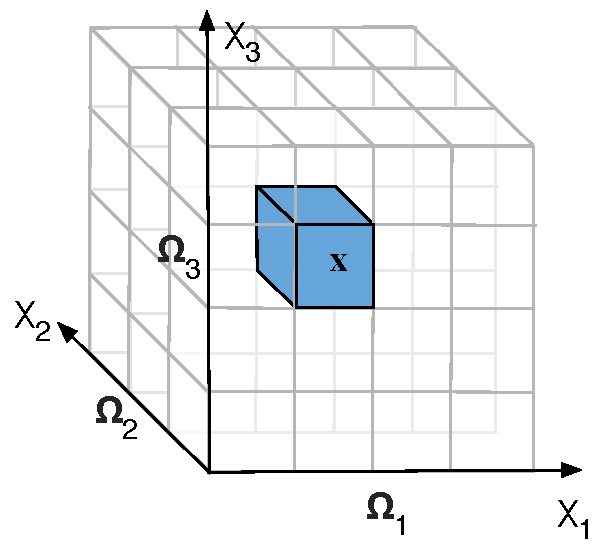
\includegraphics[width=0.6\columnwidth]{images/3Dtest}
\caption{Example of view with three discrete variables $V = \{X_1, X_2, X_3\}$.
The average divergence of the cells $\delta(\mathbf{x})$ equals the strength of
the view  $\sigma(V)$.}
\label{fig:binningexample}
\end{figure}
In fact, strength and divergence are closely connected.  Consider a view $V$.
If $V's$ dimensions are continuous, we bin them. If we compute the divergence
of each tuple and average the results, we obtain the $V$'s strength. We illustrate
this property with Figure~\ref{fig:binningexample}.  Therefore, strength and
divergence are ``two sides of the same coin''. We formalize this property it
with the lemma below.
\begin{lemma}
    If $V$ is a view with $d$ discrete variables and $\mathbf{x} \in \Omega_1
    \times \ldots \Omega_D$ is a tuple from this view, then:
    \begin{equation}\label{eq:coin}
        \sigma(V) = \mathbb{E}_{\mathbf{x}}  \big[ \delta(\{\mathbf{x}\}) \big]
    \end{equation}
\end{lemma}
\begin{proof}
    By definitions of the KL divergence, we have 
    $I(\mathbf{x} ; \rv{T})= \mathbb{E}_{\mathbf{x}}[ KL( T \parallel T |
    \{\mathbf{x}\} )]$.
    Substituting the left side with Equation~\ref{eq:strength}, and the right
    side with Equation~\ref{eq:divergence}, we obtain the lemma.
\end{proof}
Suppose that we obtained a view $V^*$ by discretizing a set of continuous
variables $V$. The average divergence of the bins equals the strength of $V^*$,
but not that of $V$. Luckily, these quantities converge as the bins get small.
\begin{lemma}
    The view $V$ is a set of continuous variables, $V^b$ is a discretized
    version of $V$ in which each variable is binned with bin size $b$, and
    $\mathbf{x}^b$ is a tuple from $V^b$. We have $\mathbb{E}_{\mathbf{x^b}}
    \big[ \delta(\{\mathbf{x^b}\}) \big] \to  \sigma(V)$ as $b \to 0$.
\end{lemma}
\begin{proof}
    Let the $D$-dimensional random vector $\mathbf{X}$ describe the
    (continuous) variables of $V$, and $\mathbf{X}^b$ describe the (discrete)
    variables of $V^b$. By generalizing Cover and Thomas, Theorem
    8.3.1~\cite{cover2012elements}, we infer that $H(\mathbf{X}^b) + D.\log{b}
    \to H(\mathbf{X})$ as $b \to 0$ .  Thus, using Equation~\ref{eq:mut-inf},
    we have $I(\mathbf{X}^b, \rv{T}) \to I(\mathbf{X}, \rv{T})$. We conclude
    that $\sigma(V^b) \to \sigma(V)$. We apply Equation~\ref{eq:coin} to obtain
    the lemma.
\end{proof}

\subsubsection{Problem Formulation}

We can now formulate our problem:
\begin{problem}
Consider a dataset $DB$, a target column $T$ and a triplet $(K, D, P)$. Find
the top $K$ strongest views with at most $D$ columns. For each of these
views, find the top $P$ divergent POIs.
\end{problem}
To solve this problem, Claude operates in two steps. First, it detects $K$
strong sets of columns.  We call this step \emph{column search}.  Then, it
extracts $P$ POI for each view. This is the \emph{POI dectection} step.

\section{Column selection}
\label{sec:colum}

{\color{red} 
This section requires some reordering.
\begin{itemize}
    \item Introduce Lemma 2, and the idea to search for columns greedily
    \item Present the exact approach
    \item Present the approximation
\end{itemize}
Also, the description of the approximation should be deepened.
}

The aim of this phase is identify the $K$ strongest sets of variables. From
here on, we assume that all the variables are discrete, and we use the
notations $D_n$ and $\rv{D}_n$ interchangeably - we can use the context to
distinguish database columns and random variables.

\subsection{Base algorithm}
\begin{figure}[t!]
\centering
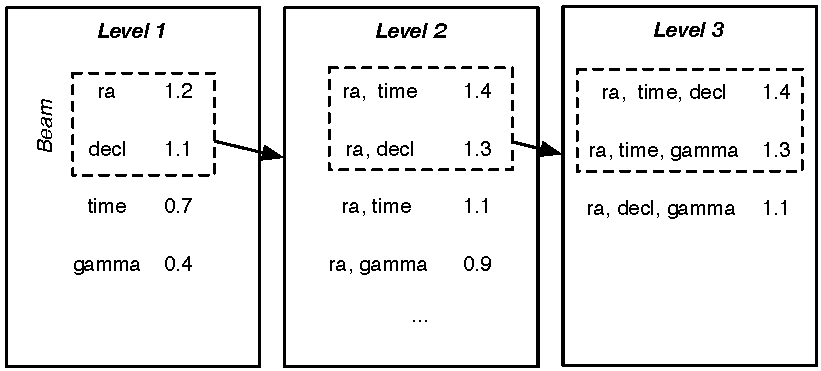
\includegraphics[width=0.8\columnwidth]{images/beam-search}
\caption{Example of Beam Search, with a beam size of 2}
\label{pic:beam-search}
\end{figure}

To recommend views, Claude must find the best sets of at most $D$ variables.
The search space of this problen grows exponentially with $D$: from a database
with $N$ variable, we can generate $\sum_{n \leq N} \binom{N}{n}$ combinations.

We propose to use level-wise search. To initialise the algorithm, we compute
the strength of each variable separately, i.e., we compute $\sigma(D_n) =
I(D_n; T)$ for every $n \in [1, N]$. We order the candidates, and keep the top
$B$ variables. We call this set the \emph{beam}. We then form new candidates by
appending each variable of the database to each variable in the beam. We obtain
views with two columns. We keep the best $B$ view, and discard the others. We
obtain a new beam.  The procedure is repeated until the beam contains views
with $D$ variables. We illustrate the procedure in Figure
\ref{pic:beam-search}.

\begin{figure}[t!]
\centering
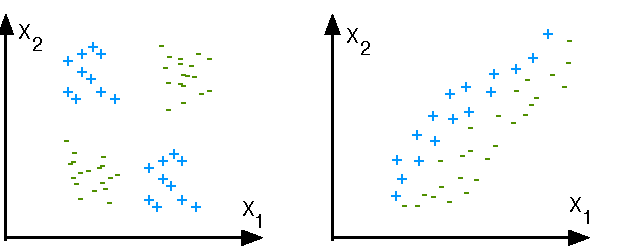
\includegraphics[width=0.8\columnwidth]{images/strength-jump}
\caption{Limit cases of the beam search strategy. The variables $var1$ and
$var2$ represent two dimensions. The symbol and color of the plots represent
the value of the target class. }
\label{pic:strength-jump}
\end{figure}
Thanks to our beam strategy, we avoid exploring an exponentially large search
space. Instead, we compute the strengths of at at most $N.B$ settings.
Unfortunately, this strategy induces an accuracy penalty: if the beam is too
small, we may miss some good candidates. This is a consequence of the following
observation: a set of columns which is outside the top $B$ candidates at step
$i$, could very well appear in the top $B$ at step $i+1$. Consider for instance
the two classic scenarios pictured in Figure \ref{pic:strength-jump}. The
dimensions $var1$ and $var2$ taken in isolation are weak: we can infer no
useful information about the target from either of them. However, their
combination is very interesting.  This observation is reflected by the
strength: the views $\{var1\}$ and $\{var2\}$ have a very poor strength, but
$\{var1, var2\}$ is an excellent candidate. If use a beam search strategy, we
may discard  $\{var1\}$ and $\{var2\}$ early because they have a low score.
This would be a mistake, because we lose the opportunity to discover $\{var1,
var2\}$.

\subsection{Approximating the View Strength}
\label{sec:approx}

The Beam Search aslgorithm gives us a convenient way to find good views.
Through the size of the beam, we can find a compromise between execution time
and accuracy.  Nevertheless, the algorithm is still too heavy for an
interactive application. For each candidate, it computes the mutual information
between all the variables of the view and the target, which involves heavy grouping
operations. Our solution is to \emph{approximate} the strength of the views
during the iterations of the algorithm. Then, we use exact calculations for the
final ranking.

To present our approximation scheme, we must first describe how a
view is impacted when we add a column to it.

\begin{lemma}\label{lem:chain}
Consider a view $V = \{D_1, \ldots, D_i\}$, and a target $T$.
For any column $D_{i+1}$: 
$$
\sigma(V \cup \{D_{i+1}\}) =  \sigma(V) + I(D_{i+1} ; T | D_1 , \ldots, D_i)
 $$
\end{lemma}
\begin{proof}
This lemma is a direct consequence of the Mutual Information's chain rule
\cite{cover2012elements}.
\end{proof}

This lemma describes how much a view improves if we append a new dimension.
For any random variables $X,Y,Z$, the notation $I(X;Y|Z)$ expresses the
\emph{conditional mutual information}. It describes the dependency between $X$
and $Y$, \emph{given $Z$}. The influence of $Z$ can go either way: it can
weaken or strengthen the relationship between $X$ and $Y$. In any case, it is
positive or null, and it is bounded by the entropy of $X$ and $Y$.

In practive, computing $ I(D_{i+1} ; T | D_1 , \ldots, D_i)$ is not less
expensive than calculating the strength of $\{D_1, \ldots, D_{i+1}\}$ directly.
But we can use the following approximation:
\[
\begin{split}
    \sigma(V \cup \{D_{i+1}\}) & = \sigma(V)   + I(D_{i+1} ; T | D_0, \ldots, D_{i})\\
                           & \approx \sigma(V) + I(D_{i+1} ; T | D_{i})
\text{ for } D_i \in V
\end{split}
\]

The idea behind this approximation is naive: we assume that $I(D_{i+1} ; T |
D_0, \ldots, D_{n}) \approx I(D_{i+1} ; T | D_{i})$. We ignore the high order
dependencies. Thanks to this assumption, we can compute the strength of a view
much faster.  Consider a directed graph in which each vertex represents a
variables $D_i$. Each edge $(D_i, D_{i+1})$ has a a weight $ I(D_{i+1} ; T |
D_{i})$.  We call this graph \emph{co-dependency} graph.  To compute the
approximate strength of ${D_0, \ldots, D_i}$, we build a spanning tree which
covers all the vertices of the view, and sum the weights of the edges.

In most cases, we can build several different spanning trees with different
weights. Which one should we use? We could use two variants. An
\emph{optimisic} approximation $\sigma_+ $ would consider the \emph{maximum}
spanning tree.  A \emph{pessimistic} approximation $\sigma_- $ would use the
weight of the \emph{minimum} spanning tree. For the rest of this paper, we will
only consider the latter alternative. 

We now present a faster version of our view search algorithm.  We operate in
two steps. First, we compute the strength of every column and every couple of
columns.  This gives us a first set of candidates, and we can derive the
co-dependency graph using the fact that $I(D_{j} ; T | D_i) = \sigma(D_i ;
D_{j}) - \sigma(D_i)$.  Then, we run Beam Search as previously, but with the
approximate strength computation.  To append the variable $D_i$ to the view
$V$, we list every edge which connects  $D_i$ to the columns of $V$. We
identify the lightest one and add the value of its weight to $\sigma(V)$.  

This algorithm is much faster because it spares us expensive database
operations. Instead, we perform computations on a graph with $d$ nodes.  To
save some accuracy, we use the exact version of the view strength for the final
top $q$ ranking.

\subsection{Deduplication}

TO DO

\section{Detecting Points Of Interest}
\label{sec:detec}

During this phase, we find the $r$ most divergent regions for each view.
Fortunatly, this task is an instance of a known Data Mining problem,
\emph{Subgroup Discovery} \cite{klosgen1996explora}\cite{wrobel1997algorithm}.
The aim of Subgroup Discovery is to identify sets for which the target value
maximizes a user-defined quality measure. To solve our problem, we instantiate
the quality measure with the divergence.

In principle, we could use any efficient algorithm from the Subgroup Discovery
litterature.  We propose to reuse the beam Search strategy from the previous
section, but to explore \emph{tuples} instead of columns. We bin the data in a
coarse manner and get a first set of $b$ cells. We then refine these cells with
a thinner binning, etc...

As mentioned in the Subgroup Discovery litterature \cite{van2011non}, our
divergence score has a drawback: it favours smaller groups.  Therefore, Beam
Search may converge very late or not at all.  A practical
solution is to alter the model to take the size into account. Let $R$
represents a range with cover $|R|$, and $|V|$ represent the number of tuples
in the view. We use the \emph{weighted} deviation $\delta_w(R) = |R|/|V| \times
\delta(R)$. This new score introduces a penalty for small POIs.


\section{Experiments}
\label{sec:experiments}

\begin{table}
    \centering
    \small
    \begin{tabular}{r c c c c} 
        \hline
        Dataset & Columns & Rows & \#Views & \#Variables\\
        \hline
        MuskMolecules & 167 & 6,600 & 22 & 18\\
        Crime & 128 & 1,996 & 20 & 17\\
        BreastCancer & 34 & 200 & 10 & 13\\
        PenDigits & 17 & 7,496 & 9 & 10\\
        BankMarketing & 17 & 45,213 & 11& 8\\
        LetterRecog & 16 & 20,000 & 10 & 12\\
        USCensus & 14 & 32,578 & 10 & 7\\
        MAGICTelescope & 11 & 19,022 & 1 & 10\\
        \hline
    \end{tabular}
    \caption{Characteristics of the datasets. The last two columns are used for
    comparison with 4S, cf. Section~\ref{sec:exp-view-selection}.}
    \label{tab:datasets}
\end{table}
We now present our experimental results. All our experiments are based on 8
datasets from the UCI Repository, described in Table~\ref{tab:datasets}. The
files are freely available online\footnote{archive.ics.uci.edu/ml/}.

\subsection{Detailed Example: Crimes in the US}
\label{sec:crime}

\begin{table}[t]
  \centering
  \small
  \rowcolors{2}{gray!25}{white}
  \begin{tabulary}{\columnwidth}{L c}
    \hline
    View & Score (normalized)\\
    \hline
    Police.Overtime, Pct.Vacant.Boarded, Pct.Race.White & 0.51\\
    Pct.Families.2.Parents, Pct.Race.White, Police.Requests.Per.Officer & 0.49\\
    Pct.Police.White, Pct.Police.Minority, Pct.Vacant.House.Boarded& 0.37\\
    Pct.Empl.Profes.Services, Pct.Empl.Manual, Pct.Police.On.Patrol & 0.37\\
    Pct.Retired, Pct.Use.Public.Transports, Pct.Police.On.Patrol& 0.35 \\
    Pct.Recently.Moved, Population.Density, Police.Cars & 0.34 \\
    \hline
\end{tabulary}
    \caption{Example of views generated by Claude for the US Crime dataset.}
    \label{tab:crime_views}
\end{table}
\begin{figure}[t!]
    \centering
    \begin{subfigure}[b]{0.4\columnwidth}
    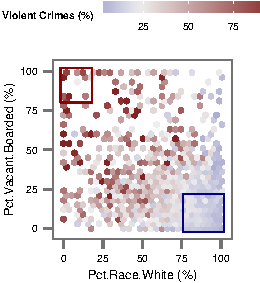
\includegraphics[width=\textwidth]{plots/crime1}
    \end{subfigure}
    \begin{subfigure}[b]{0.4\columnwidth}
    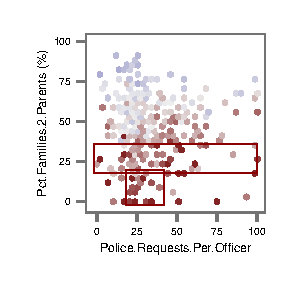
\includegraphics[width=\textwidth]{plots/crime2}
    \end{subfigure}

    \begin{subfigure}[b]{0.4\columnwidth}
    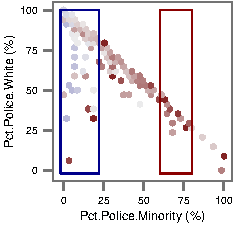
\includegraphics[width=\textwidth]{plots/crime3}
    \end{subfigure}
    \begin{subfigure}[b]{0.4\columnwidth}
    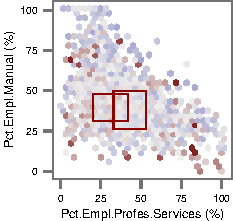
\includegraphics[width=\textwidth]{plots/crime4}
    \end{subfigure}
    
    \begin{subfigure}[b]{0.4\columnwidth}
    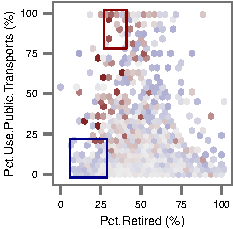
\includegraphics[width=\textwidth]{plots/crime5}
    \end{subfigure}
    \begin{subfigure}[b]{0.4\columnwidth}
    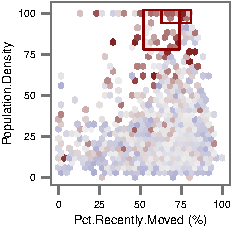
\includegraphics[width=\textwidth]{plots/crime6}
    \end{subfigure}
\caption{Heatmaps of the US Crime Dataset, based on Claude's output. Each box
represents a Point of Interest.}
\label{pic:crime_charts}
\end{figure}

In this section, we showcase Claude with a real-life example: we analyze the
Communities and Crime dataset form the UCI
repository\footnote{archive.ics.uci.edu/ml/datasets/Communities+and+Crime}.
Our aim is to understand which US cities are subject to violent crimes. Our
database compiles crime data and socio-economic indicators about 1994
communities, with a total of 128 variables. The data comes mostly from the
90's, and it was provided by US government sources - among others, the 1990 US
census and the 1995 FBI Uniform Crime Report. All the variables are
normalized to have a minimum of 0 and a maximum of 100.

We generated $K=100$ explanations with up to $D=3$ dimensions, both with and
without deduplication. We present a selection of explanations in
Table~\ref{tab:crime_views}, along with 2-dimension heatmaps in
Figure~\ref{pic:crime_charts}. Observe that strong views have a visual
signature: in the top two maps, the blue and red areas are neatly separated. In
the bottom two views, the distinction is less clear.

The first view of Table \ref{tab:crime_views} is the best one we found:
\texttt{Police. Overtime, Pct.Race.White, Pct.Vacant.Boarded}. It has a score
of 0.51. which means that these three variables contain 51\% of the target's
information. The columns \texttt{Police. Overtime} and \texttt{Pct.White.Race}
respectively describe the average time overworked by the police and the
percentage of caucasian population. The third variable,
\texttt{Pct.Vacant.Boarded} was surprising to us: it describes the
percentage of vacant houses which are boarded up.  How does this relate to
crime? We could assume that boarded houses are associated with long term
abandon, and thus, poverty. The top-left plot of Figure \ref{pic:crime_charts}
shows the relation between race, boarded houses and crime. Observe that the
variables complement each other: a high proportion of caucasians may or may not
lead to low crime. However, a high proportion of caucasians \emph{combined
with} a low rate of boarded house correspond to safe areas, while little
caucasians and many boarded houses correspond to more violent communities.

Our second view shows that cities with more monoparental families tend to be
more violent: the correlation is clearly visible, and both POIs point to the
bottom of the chart. However, close inspection also reveals surpsises: a few
communities have a relatively high number of two-parents families, but also
high indicators of police requests and crime (in the top right corner of the
chart). Manual queries reveals that many of these cities are located in the
suburbs of Los Angeles, and contain a majority of Hispanics. Does this explain
the peculiarity? We leave this question open for future investigations. We see
that some findings come from the recommendations directly while others are
serendipitous.  But in both cases, Claude lets us discover ``nuggets'' with
little prior knowledge and few assumptions. 

\subsection{View Strength and Prediction}
\label{sec:view-strengh}

\begin{figure}[t!]
\centering
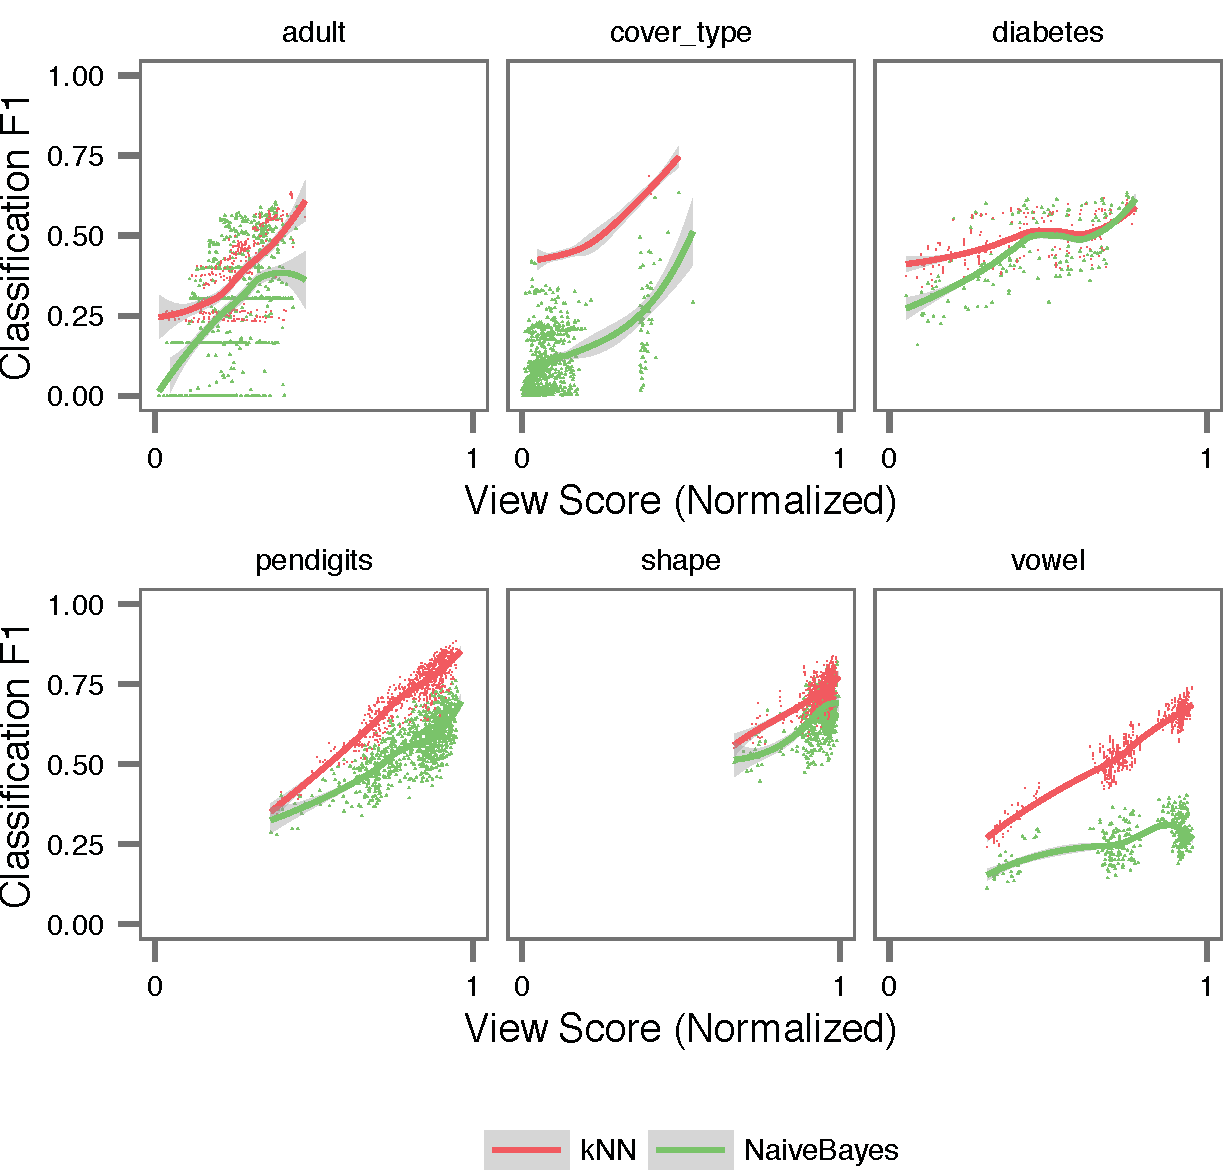
\includegraphics[width=\columnwidth]{plots/compare-strength-f1}
\caption{Strength vs. Classification accuracy for 500 random views. The blue
and red lines were obtained by linear regression.}
\label{pic:strength-vs-f1}
\end{figure}
In this section, we show experimentally that our notion of view strength
``works'', e.g. that strong views effectively provide information about the
target column. To verify this assumption, we simulate users with statistical
classifiers. Consider a view $V$ over a database. If a classifier can predict
the value of the target from $V$'s columns, then $V$ is informative.
Oppositely, if the classifier fails, then $V$ is potentially uninteresting. In
other words, we should observe a positive correlation between views strength
and classification accuracy.

We now detail our experiment. We chose three datasets from the UCI repository.
For each dataset, we generated 500 random views and measured their strengths.
We then trained classifiers on each of these views, and measured their
performance. We report the results in Figure \ref{pic:strength-vs-f1}. We chose
two classification algorithms: Naive Bayes, and 5-Nearest Neighbors.  We chose
those because they contain no built-in mechanism to filter out irrelevant
variables (as opposed to, e.g., decision trees). We measure the classification
performance with 5-fold validation, to avoid the effects of overfitting.

In all three cases, we observe a positive correlation between the strengths of
the views and the accuracy of the predicictions. We confirm these observations
with statistical tests: the coefficients of determination ($R^2$) vary between
0.11 and 0.84, which indicates the presence of a trend (despite some
variablity). Furthermore, the p-values associated to the coefficients are all
under $10^{-3}$, this gives us excellent confidence that the strength
influences positively the prediction accuracy. In conclusion, strong views are
indeed more instructive.


\subsection{View Selection}
\label{sec:exp-view-selection}

We now evalute Claude's output and runtime in detail. In this section, we
verify if Claude's algorithm produces good views in a short amount of time. To
do so, we compare it to four methods, three of which come from the machine
learning litterature.  Our first baseline, \texttt{Exact}, is similar to
Claude, but we removed the approximation scheme presented in \ref{sec:approx} -
instead we compute the exact mutual information between the views and the
target. The method should be slower, but more accurate. 

The second algorithm, \texttt{Clique}, is a top-down approach inspired by
recent work on pattern mining~\cite{xie2010max}. The idea is to build a graph
where each vertex $i$ represents a column $D_i$, and each edge $(i,j)$
represents the view $\{D_i, D_j\}$. We then simplify the graph: we keep the
edges associated with the top $B$ strongest views, and we eliminate all the
others. To detect strong views with $D >2$ variables, we seek cliques in this
degenerated graph. We used the \texttt{igraph} package from R. We expect this
algorithm to be very fast, but less accurate.

The third method, \texttt{Wrap 5-NN}, is a classic feature selection
algorithm~\cite{guyon2003introduction}. The idea is to train a 5-Nearest
Neighbour classifier with increasingly large sets of variables. We first test
each variable separately, and keep the column which led to the best prediction.
Then we keep adding variables in a Breadth-First manner, until the
quality of the predictions stops increasing or we reach $n$ variables. Our
implementation is based on the \texttt{class} package from R.  We modified the
original algorithm to maintain and update $q$ distinct sets of variables
instead of just one. We chose the nearest neighbour algorithm because it is
fast, and it gave us good performance, as shown in \ref{sec:view-strengh}. We
expect this algorithm to be very slow, but close to optimal.

Finally, the last method, \texttt{4S} is a state-of-the-art subspace search
method from the unsupervised learning literature~\cite{nguyen20134s}. The aim
of the algorithm is to detect ``interesting'' subspaces in large databases,
independantly of a target variable. To do so, it seeks groups of variables
which are mutually correlated, with sketches and graph-based techniques.  We
used the author's implementation, written in Java. We expect the algorithm to
be very fast and reasonably accurate.

We use 8 public datasets, presented in Section \ref{sec:experiments}. For a
fair comparison, we must ensure that each algorithm generates the same number
of views ($K$) with the same number of variables ($D$).  However, we have no
way to specify these parameters a priori with 4S, because the algorithm has a
built-in mechanism to pick optimal values. Therefore, we run 4S first on each
dataset, we let it chose $K$ and $D$, and we use these values for the remaining
algorithms.  We report the obtained parameters in Table~\ref{tab:datasets}.

We implemented Claude in R, except for some information theory primitives
written in C. For practical reasons, we interupted all the experiments which
lasted more than 1 hour. Our test system is based on a 3.40 GHz Intel(R)
Core(TM) i7-2600 processor. It is equipped with 16 GB RAM, but the Java heap
space is limited to 8 GB. The operating system is Fedora 16. 

\begin{figure*}[t!]
\centering
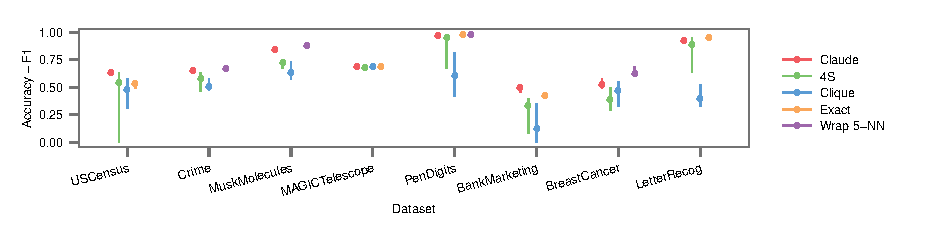
\includegraphics[width=2\columnwidth]{plots/view-scores}
\caption{Performance of the View Selection algorithms. For each data set, we
    generate $q$ views, train a 5-NN classifier over the columns of each view
    and report the classification accuracy (F1, 5-fold cross validation). The
    points represent median scores, the bars represent the lowest and greatest
    scores.} 
\label{pic:column-select-score}
\end{figure*}
\begin{figure*}[t!]
\centering
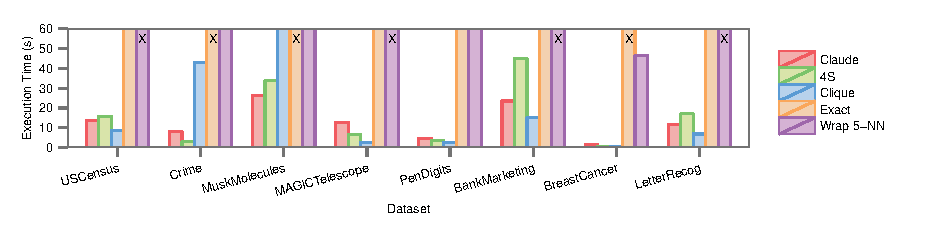
\includegraphics[width=2\columnwidth]{plots/view-times}
\caption{Execution time of the View Selection algorithms. A \texttt{X} symbol
indicates that the experiment did not finish within 3,600 seconds.}
\label{pic:column-select-time}
\end{figure*}

\textbf{Accuracy.} In Figure \ref{pic:column-select-score}, we compare the
quality of the views returned by each algorithm. For each competitor, we
generate $q$ views with $n$ variables, train a classifier on each view and
measure the quality of the predictions. For the classification, we use both
Naive Bayes and 5-Nearest Neighbors, and report the highest score.  We measure
accuracy with the F1 score on 5-fold cross validation; higher is better.

The method \texttt{Wrap 5-NN} comes first for all the datasets on which it
completed. This is not surprising since the algorithm optimizes exactly what we
measure: \texttt{Wrap 5-NN} is our ``gold standard''. Our two algorithms,
\texttt{Claude} and \texttt{Exhaustive}, come very close. This indicates that
both algorithms find good views, and that our approximation scheme works
correctly.  The algorithms \texttt{4S} and \texttt{Clique} come much lower. As
\texttt{4S} is completely unsupervised, we cannot expect it to perform as well
as a the other approaches. The assumptions behind \texttt{Clique} are
apparently too naive.

\textbf{Runtime.} Figure~\ref{pic:column-select-time} shows the runtime of our
experiments. The algorithms \texttt{Exact} and \texttt{Wrap 5-NN} are orders of
magnitude slower than the other approaches. The remaining three approaches are
comparable: depending on the datasets, either \texttt{Clique} or \texttt{4S}
come first. Claude comes first for \texttt{MuskMolecules}, and close
second for all the other datasets. We conclude that Claude is compairable to
state-of-the-art algorithms in terms of runtime, but it generates better views.

\begin{figure}[t!]
\centering
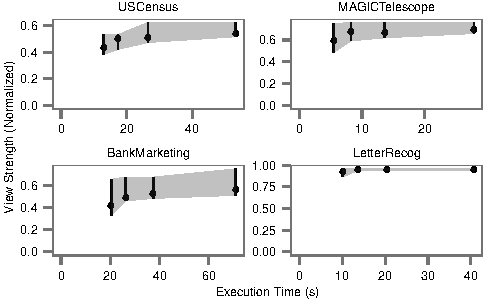
\includegraphics[width=\columnwidth]{plots/view-vary-beam}
\caption{Impact of the beam size on the execution time and view strength. For
each dataset, we generated 25 views with beam size 25, 50, 100 and 250. The
points represent the medium scores, the bars represent the lowest and greatest
scores.}
\label{pic:view-beam}
\end{figure}
\begin{figure}[t!]
\centering
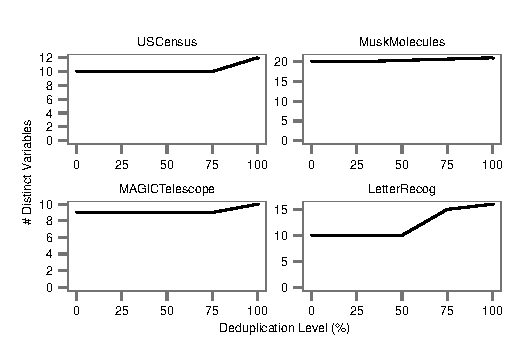
\includegraphics[width=\columnwidth]{plots/view-vary-diversification}
\caption{Impact of the deduplication. The y-axis presents the number of
distinct variables used in the top 25 views.}
\label{pic:view-diversification}
\end{figure}
\textbf{Impact of the beam size.} Figure~\ref{pic:view-beam} shows the impact
of the beam size $B$ on Claude's performance, for 4 databases. To obain these
plots, we ran Claude with $K=25$ and $D=5$, and varied $B$ between 25 and 250.
We observe that smaller beams lead to lower execution times, while larger beam
lead to stronger views. However, the heuristic converges fast: we observe
little to no improvement for $B$ greater than 50.

\textbf{Impact of the deduplication.} We show the impact of our deduplication
strategy in Figure \ref{pic:view-diversification}.  We ran Claude with $K=25$
and $D=5$, and varied the level of deduplication. To quantify the diversity of
the views, we report the number of distinct variables used. We observe that the
strategy works in all four cases, but with different levels of efficiency. In
the \texttt{LetterRecog} case, our strategy increases the number of variables
by almost 30\%. The effect is much lighter on \texttt{MuskMolecules}.

\subsection{POI Detection}
\label{sec:exp-poi}

\begin{figure*}[t!]
\centering
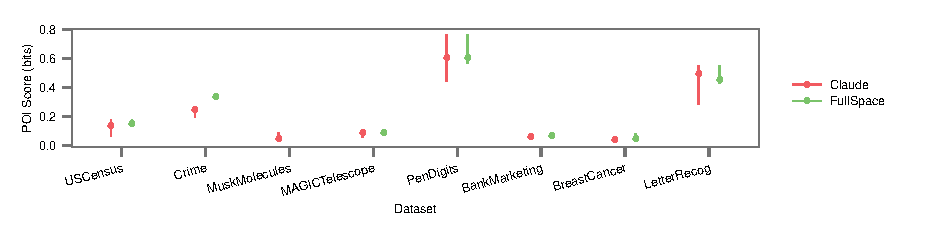
\includegraphics[width=2\columnwidth]{plots/POI-score}
\caption{Quality of the Point of Interests. For each view, we detect $P=10$
POIs. The
    points represent median scores, the bars represent the lowest and greatest
    scores.}
\label{pic:POI-quali}
\end{figure*}
\begin{figure*}[t!]
\centering
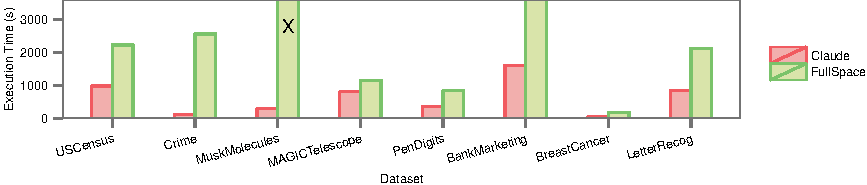
\includegraphics[width=2\columnwidth]{plots/POI-timing}
\caption{Execution time of the POI detection. A \texttt{X} symbol
indicates that the experiment did not finish within 7,200 seconds.}
\label{pic:POI-time}
\end{figure*}

In this section, we evaluate Claude's POI detection strategy. We compare two
approaches. The first approach is the algorithm presented in the paper: first
we search $K$ views, then we return $P$ POIs per view. The second approach,
\texttt{FullSpace}, is the method used in much of the recent Subgroup Discovery
litterature \cite{van2011non, duivesteijn2010subgroup}.  The idea is to apply
Beam Search on the whole database directly. Instead of seeking $P$ POIs in $K$
projections, we seek $K.P$ selections from the full column space; we skip the
view selection step. We use the same datasets as previoulsy. Our default
parameters are $K=25$, $D=5$, $B=50$ and $P=10$. To set the beam size, we use a rule of
thumb: $B_{POI} = 2.k$ ($B_{POI}$ is the beam used for POI detection,
not for view search). In order to gather sufficient data, we raise our time
limit to 2 hours. 

Figure \ref{pic:POI-quali} compares the quality of the POIs found by both
algorithms. The strategy \texttt{FullSpace} gives slightly better results on
\texttt{Crime} and \texttt{PenDigits}, but the difference is close to null. The
scores are similar on all the other datasets. We conclude that Claude's POIs
are very close to those found by a state-of-the-art Subgroup Discovery approach.
Figure~\ref{pic:POI-time} compares the runtimes of both approaches.  We observe
that Claude is much faster than \texttt{FullSpace}. The difference grows with
the number of columns: the runtimes are almost similar for datasets with few
columns (\texttt{MAGICTelescope}), but \texttt{Claude} is considerably faster
for larger databases (more than an order of magnitude difference for
\texttt{MuskMolecules}). Although this was not our initial aim, decoupling view
search and POI extraction allows us to find subgroups faster in high dimension
datasets.

\section{Related Work}
Our work is inspired by both database research and machine learning. On the
database side, Claude is related to the \emph{query recommendation} problem:
how to automatically generate interesting SQL queries for a given database? On
the machine learning side, our work is based on \emph{feature selection}, e.g.,
how to select variables for a given inference problem, and \emph{subgroup
discovery}, e.g., how to find the tuples which maximize a particular score
function.

\textbf{Query Recommendation.} We identify two types of recommendation systems:
\emph{human-driven} approaches and \emph{data-driven} approaches. Human-driven
systems learn from user feedback. For instance, Chatzopoulou et al. propose to
make recommendations from query logs, similarly to search engines
\cite{chatzopoulou2009query}. More recently, authors have proposed interactive
exploration systems, where a recommendation system ``guides'' the user through
the database. In Explore-by-Example, the system infers queries from examples
provided by the user \cite{dimitriadou2014explore}. With Charles, the engine
decomposes large queries into smaller ones \cite{sellam2013meet}. Sarawagi's
method builds a maximum entropy model over the database from the user's history 
\cite{sarawagi2000user}. Bonifati et al. propose a similar method to recomend
joins \cite{bonifati2014interactive}.  Claude competes with neither of these
approaches, since it uses the content of the database only.

Our work is closer data-driven data recommendation, in which the system makes
recommendations based on the content of the data. The general idea is to build
a statistical model of the database, and find regions which behave
unexpectedly. Sarawagi et al. have published seminal work on this topic for
OLAP cubes \cite{sarawagi1998discovery}. Their system highlights sequences of
drill-in operations which lead to ``surprising data'', e.g., tuples which
differ from their neighbourhood. It requires that the data is organized in an
OLAP cube (with hierchical dimensions), it supposes that the users know which
variables to use, and it seeks thin-grained deviations. Oppositely, our system
uses regular tables, it recommends views (not only selections) and it seeks
large trends. More recently, Dash et al. have proposed a method to reveal
surprising subsets in a faceted search context \cite{dash2008dynamic}. This
method is related to Claude, but it targets document search, it does not
recommend views.

\textbf{Projection Search.} cf. data viz: Grand Tour, scagnostics, etc...


\textbf{Feature Selection, Subspace Search.} Chosing which variables to use for
classification or regression is a crucial problem, for which dozens of methods
were proposed \cite{guyon2003introduction}. Similarly to Claude, some of these
methods rely on mutual information~\cite{peng2005feature} Nevertheless, the
objective is different. A feature selection algorithm seeks \emph{one} set of
variables on which a statistical predictor will perform optimally. Claude seeks
several, small sets of variables, simple enough to be interepreted by a humans.
Claude is halfway between inference and exploration.

On the unsupervised learning side, our work is close to subspace search. The
idea is detect subspaces where the data is clustered distinctly
\cite{keller2012hics,nguyen20134s}. We compare Claude to state-of-the-art
methods in our Experiments section.

\textbf{Subgroup Discovery.} Our work is very close to subgroup discovery
\cite{klosgen1996explora, wrobel1997algorithm, van2011non}. We discuss the
connections and compare approaches in Sections~\ref{sec:detec}
and~\ref{sec:exp-poi} respectively.

\section{Conclusion}

Future work: Causation models, synergy with visualisation
